% vim: set tabstop=4 shiftwidth=4 expandtab : 
\section{Motivation \label{sec:motivation}}

    % Representative inputs are important. Example.
    % Artificial representative input sets are hard to create
    % Representative input sets created out of real data are also hard to create
    % Just using real data online is not enough. Efficiency metrics are needed
    % We do not have a proper efficiency metric. Example.
    % The paper shows how to construct one. 

    In this section we first motivate online iterative compilation by showing the deleterious effects of using non-representative input
    sets and that it is hard to create representative ones. Then we go on to examine what stops us from just using real inputs online and
    what we need to overcome the problem.

    \paragraph{Iterative compilation needs representative inputs.} 
    In order to highlight what happens when we apply iterative compilation using the wrong set of inputs, we selected two distinct sets of
    10 out of the 1,000 inputs of the of \textit{KDataSets}~\cite{chen10,chen12a} for the \texttt{tiff2bw} benchmark.
    The first set represents the training set, i.e., the set of inputs that will be used for selecting the best optimization sequence by
    iterative compilation, and the second set is a specific set of inputs which is misrepresented by the training set.
    After performing iterative compilation on the first set, the selected optimization sequence has an average speedup of 1.22 over -O3 for
    the training set itself, but it produces a slowdown of 0.91 for the second set of inputs.
    However, if the iterative compilation was performed on the second set itself, it would be able to find a optimization sequence that
    produces a speedup of 1.07 over -O3.


\begin{figure}[t]
    \centering
    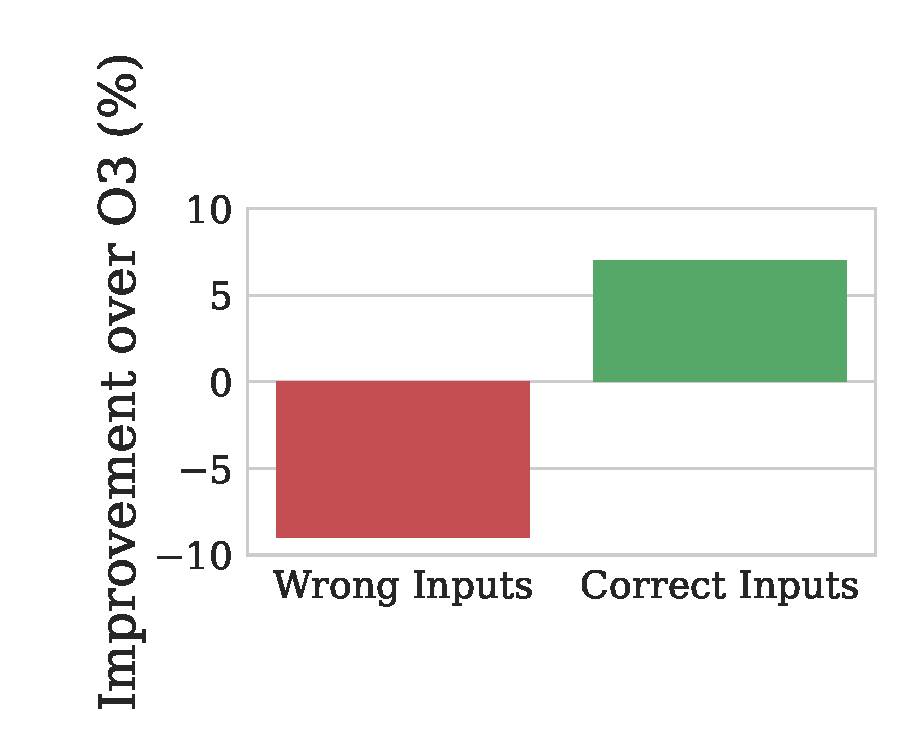
\includegraphics[width=0.7\linewidth]{figs/motivation_wrong_inputs.pdf}
    \caption{Iterative compilation performed on the wrong set of inputs compared to the ideal case for the \texttt{tiff2bw} benchmark.}
    \label{fig:motivation_wrong_inputs}
\end{figure}

    %Even with larger set of training inputs, the lack of representative inputs for iterative compilation can still hurt performance.
    %For the same \textttt{tiff2bw} benchmark, we were able to partition the whole dataset into 
    %I.C. on 85% set has speedup 1.06 on the set itself and 0.975 slowdown on the 15% set.
    %I.C. on 15% set has speedup 1.03.

%%    \paragraph{Iterative compilation needs representative inputs.} \FIXME{Fig.XXX} shows what happens when we apply iterative compilation
%%    on \FIXME{susan\_c} using the wrong inputs. We selected \FIXME{50} of the 1,000 inputs of \textit{KDataSets}~\cite{chen10,chen12a} for
%%    \FIXME{susan\_c} and we used them to evaluate different optimizations. The red bars show the average speedup over \texttt{-O3} achieved
%%    by the optimization sequence selected by iterative compilation. On the left is the average over the \FIXME{50} inputs, on the right the
%%    average over all 1,000 inputs. The selected sequence works great for the inputs we used, but it fails miserably for the rest, slowing
%%    down the benchmark by \FIXME{5\%} on average. 
%%
%%    The blue bars, on the other hand, show the ideal case where good optimizations are selected based on their average effect on all
%%    inputs, not just a subset. Not only is the average speedup over all 1,000 inputs considerable, \FIXME{13\%} over \texttt{-O3}, but it
%%    also works well for the \FIXME{50} input subset. The speedup for the subset is only \FIXME{1\%} less of what we got when we optimized
%%    specifically for that subset.
%%
%%    Making iterative compilation work in this example is not a matter of handling input sensitivity, we were able to find an optimization
%%    sequence that works well both on average and under most inputs. It is a matter of finding a set of inputs that represents the full
%%    range of inputs the application is likely to process. If we do, we can improve average performance by \FIXME{13\%}. If not, we might
%%    hurt average performance instead. 
    
    \paragraph{Representative input sets are hard to create.} For developers to create artificial input sets, they first need to know how
    their application is actually being used. This is not always easy or even possible. Then, they need to create data that will trigger a
    similar behavior and this needs a deep knowledge of the application and considerable effort. This will have to be a continuous work in
    progress, to handle changes in the way the application is used.

    Collecting real input data online and processing them again offline to evaluate optimizations is not a solution either. It requires
    manual modifications to the application to save the data, more modifications to avoid side effects while reusing data, and even more
    modifications to ensure that the application does the same work every time the same data are reused, despite changes in the rest of
    the system state. This is significant engineering work. Even if this was not the case, many applications are just not able to save
    data for privacy or storage overhead reasons.
    
    %\paragraph{Using real inputs online is not enough.} We could overcome these problems by just evaluating optimization sequences online
    %while the application is being used. This gives us live data but creates a new problem. Optimization sequences are compared based on
    %how much faster the program becomes. When all of them are tested against the same inputs, it is just a matter of comparing runtimes.
    %A shorter runtime for processing the same data means a more efficient binary. With live data, we cannot do this, each binary processes
    %whatever the input happens to be. We need another efficiency metric that only requires a single use of an optimized binary with a
    %single input.

    \paragraph{Challenges of using real inputs online.} We could overcome the problems of representative inputs by just evaluating
    optimization sequences online while the application is being used. 
    %Optimization sequences are compared based on how much faster the program becomes.
    This gives us live data but creates a new problems.
    With live data, we cannot just compare runtimes. 
    When all of the optimization sequences are tested against the same inputs, it is just a matter of comparing runtimes.
    A shorter runtime for processing the same data means a more efficient binary.
    With live data, we cannot do this, each binary processes
    whatever the input happens to be. We need another efficiency metric that only requires a single use of an optimized binary with a
    single input.

    \paragraph{Existing efficiency metrics are not up to the task.} Application-specific efficiency metrics~\cite{alameldeen06,coppa14} may
    work well, but the developer has to choose the appropriate metric and then manually modify the application to calculate it. Speedup
    over a common baseline binary is a good application-agnostic metric, equating efficiency with how much faster a given input is
    processed. It would be ideal, if we did not have to use the same input twice, one with the baseline and one with the optimized binary.
    
    Typical single-run performance metrics, like runtime or Instructions Per Cycle~(IPC), are not fit for purpose. To show this, we ran
    each of the \FIXME{32} \textit{KDataSets} benchmarks 1,000 times, each time with a different input \textit{and} a different optimized
    binary, and we measured three metrics: runtime, inverse runtime, and IPC. \FIXME{Fig.XXX} shows the correlation coefficient between
    them and a reasonable efficiency metric, speedup over \texttt{-O0}. For all benchmarks, the correlation coefficient is below
    \FIXME{0.20} for runtime and below \FIXME{0.35} for inverse runtime. Both have obvious reasons for being inappropriate efficiency
    metrics. Doubling the amount of data to be processed will cause the runtime to rise and the inverse runtime to fall, even if we use the same binary.
    Efficiency has nothing to do with it. IPC also correlates poorly with efficiency, the correlation coefficient being just \FIXME{0.15}.
    While it is used often in computer architecture, it works there because it is used with invariant binaries. In contrast, any compiler
    optimization that trades high latency instructions for multiple low latency instructions can reduce IPC while improving efficiency.
    
    No existing metric can give us an application-agnostic measure of efficiency with a single execution. The rest of the paper will show
    how to create one and how to use it for iterative compilation. 


\begin{figure*}[t]
    \centering
    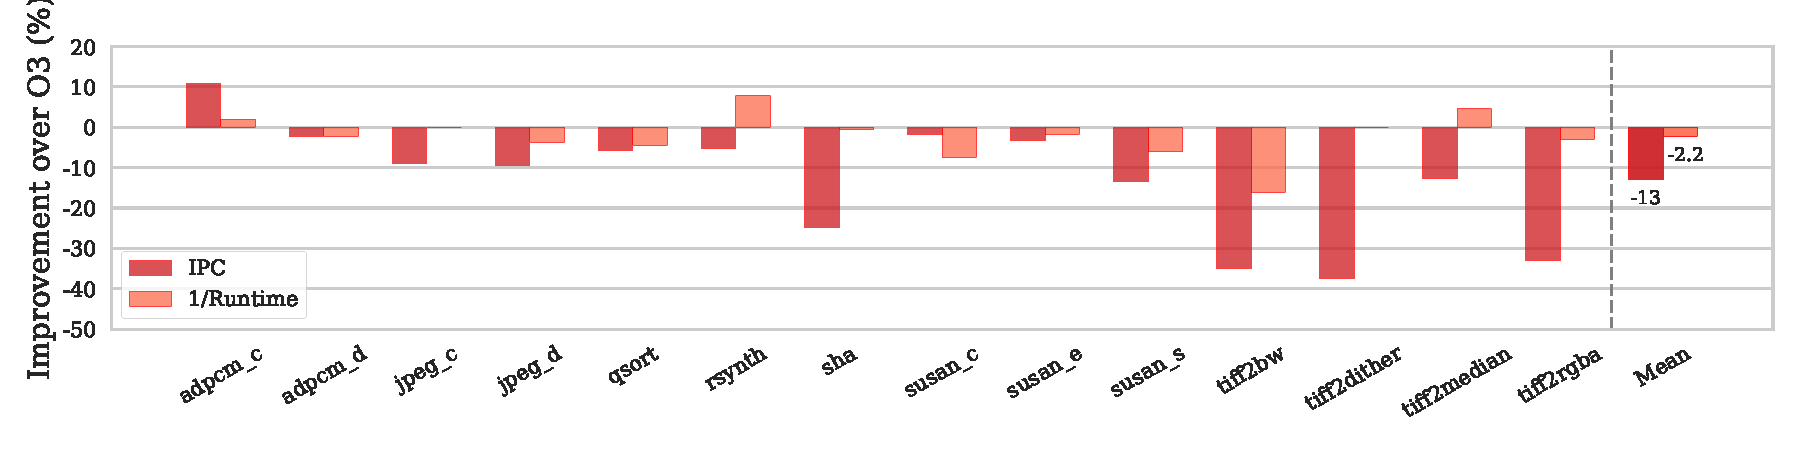
\includegraphics[width=\textwidth]{figs/motivation-speedups.pdf}
    \caption{\FIXME{[Fall-back Result]} Performance improvement of iterative compilation guided by IPC and runtime.}
    \label{fig:motivation-speedups}
\end{figure*}

